\documentclass[12pt]{beamer}
\usetheme{Boadilla}
\usepackage{graphicx}
\usepackage{algorithm2e}
\graphicspath{{images/}}
\title{CMPT 155: Computer Applications for Life Sciences}
\subtitle{Lecture 2: Navigating Through Excel}
\author{Ivan E. Perez}
\institute{}
\date{January 21, 2022}
\usepackage{booktabs} % Allows the use of \toprule, 
\usepackage{appendix}
\usepackage{enumerate,multicol}
\usepackage{amsmath, amssymb, amsthm}
\usepackage{tikz}

\begin{document}
	\begin{frame}
		\titlepage
	\end{frame}
	
	\begin{frame}
		\frametitle{Presentation Outline}
		\tableofcontents
		
	\end{frame}
	
	\section{Navigating Excel}
	
	\begin{frame}
		\frametitle{Starting a Workbook}
		\begin{itemize}
			\item an Excel \textcolor{red}{workbook} file is a collection of one or more worksheets and takes on the extension .xlsx
			\item When you open excel it typically starts a workbook named ``Book1".  
		\end{itemize} 
		\begin{center}
			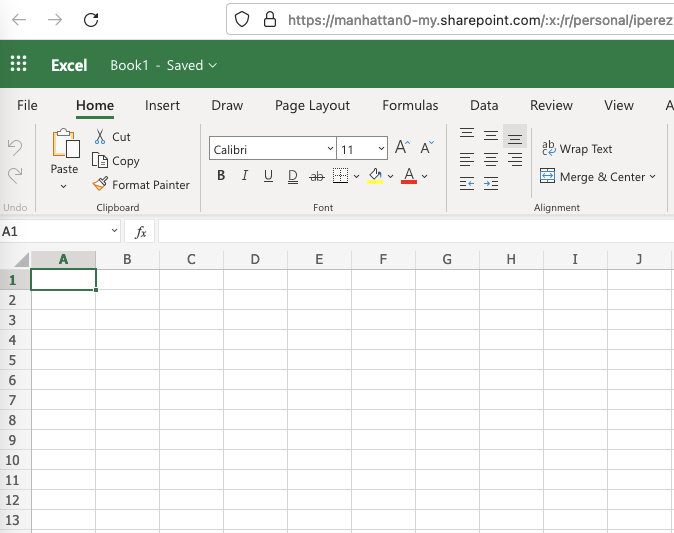
\includegraphics[width=10cm]{Workbook.png}
		\end{center}
	\end{frame}
	
	\begin{frame}
		\frametitle{The Ribbon}
		\begin{itemize}
			\item Everything that happens in Excel can be easily accessed through \textbf{The Ribbon}			
		\end{itemize}
		\begin{center}
			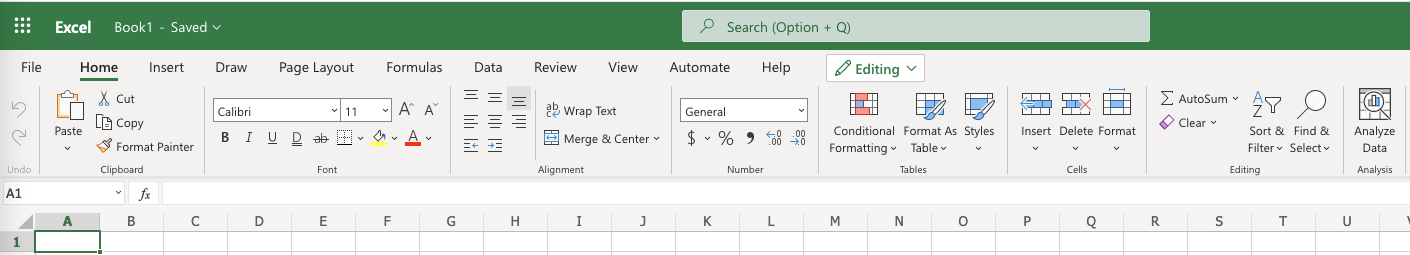
\includegraphics[width=10cm]{Ribbon.png}
		\end{center}	
\end{frame}
	
	\begin{frame}
		\frametitle{File Options \& Backstage View}
		By clicking on the 
		\begin{itemize}
			\item show an image of file options
		\end{itemize}
		\begin{center}
			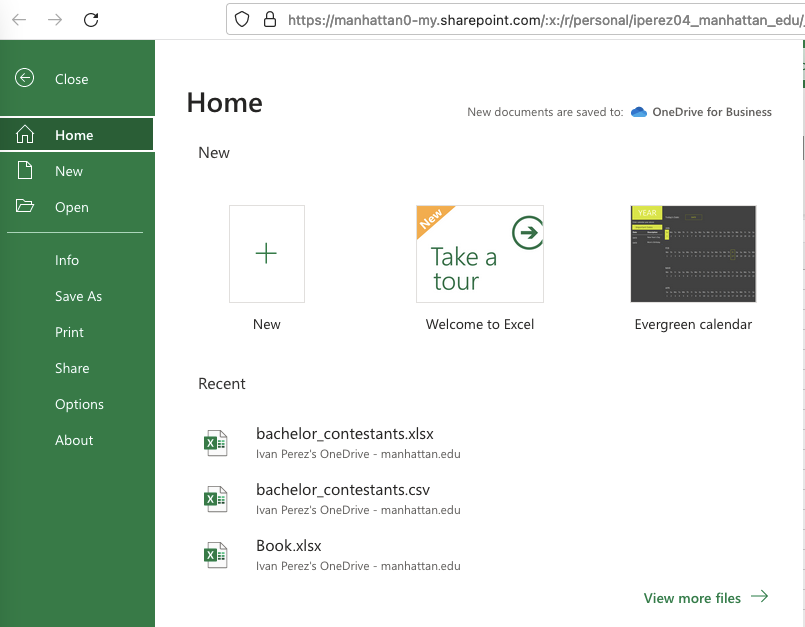
\includegraphics[width=10cm]{FileTab.png}
		\end{center}	
\end{frame}

	\begin{frame}
		\frametitle{Worksheet Basics}
		\begin{itemize}
			\item The grid vidides your worksheet into rows (1,2,3)
			and columns (A, B, C, \ldots).
			\item the smallest unit in a worksheet is the \textcolor{red}{cell} (C2, F6, \ldots).
			\item A Worksheet can contain a maximum of 1 million rows, and 16,000 for 16 million unique pieces of data!
			\item add an annotated sheet of your column cells.
		\end{itemize}
	\end{frame}
	
	\begin{frame}
		\frametitle{Column Titles/Headers}
		\begin{center}
		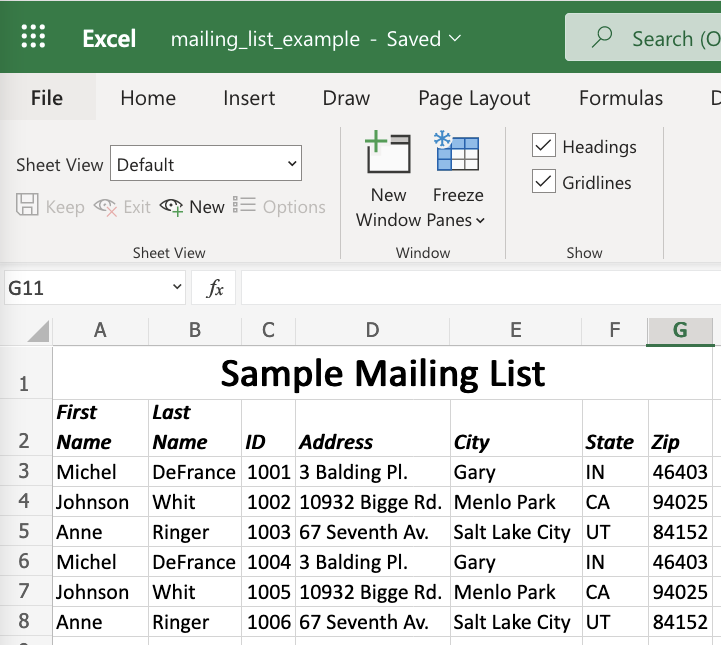
\includegraphics[width=10cm]{ExampleWorkbook}
		\end{center}
	\end{frame}

	\begin{frame}
		\frametitle{Adding Data}
		Let's try adding data to a blank workbook!
		\begin{itemize}
			\item Michael DeFrance, 3 Balding Pl., Gary, IN 46403
			\item Johnson Whit, 10932 Bigge Rd., Menlo Park, CA 94025
			\item Anne Ringer, 67 Seventh Av., Salt Lake City, UT 84152
		\end{itemize}
		lets try:
		\begin{enumerate}
			\item Make the column titles bold
			\item Adjust the width of the columns to fit content
		\end{enumerate}
	\end{frame}
	
	\begin{frame}
		\frametitle{Editing Data}
		Cells can be edited by first selecting a cell with your cursor or arrows
		\begin{itemize}
			\item directly typing to replace the text in the cell
			\item double clicking to edit text. 
		\end{itemize}
		Delete/clear cells by selecting and pressing del / backspace keys. \\
		Navigating through cells: \begin{itemize}
			\item press  `Tab' to move selection one cell to the right
			\item press `Enter' to go to the next line.
			\item use arrow keys/mouse to move selection 
		\end{itemize}
	\end{frame}
	\begin{frame}
		\frametitle{Common Keyboard Shortcuts/key bindings}
			\begin{tabular}{|l|l|l|}
				\hline
				Shortcut Win & Shortcut Mac & Effect \\
				\hline
				Ctrl + C & Cmd + C & Copy Selection \\
				Ctrl + X & Cmd + X & Cut Selection \\
				Ctrl + V & Cmd + V & Paste Selection\\
				Ctrl + S & Cmd + S & Save File \\
				Ctrl + Shift + S & Cmd + Shift + S & Save As... Filetype \\ 
				Ctrl + O & Cmd + O & Starts Open File Dialogue \\
				Ctrl + N & Cmd + N & Start New Blank workbook \\
				Ctrl + F & Cmd + F & Open Find \& Replace\\
				Ctrl + Z & Cmd + Z & Undo \\
				Ctrl + Y & Cmd + Y & Redo \\
				\hline
			\end{tabular}\\
		\bigskip
		Try using these shortcuts at least once so you see what they do!\\
		\textcolor{blue}{\href{https://support.microsoft.com/en-us/office/keyboard-shortcuts-in-excel-1798d9d5-842a-42b8-9c99-9b7213f0040f}{Link to a more comprehensive list of keyboard shortcuts for excel}}
	\end{frame}
	\begin{frame}
		\frametitle{Exercise}
		Lets Try to build a simple expense worksheet from the data given below:\\
		\begin{center}
			\begin{tabular}{ |l|l|l|}
				\hline
				Date Purchased & Item & Price\\
				\hline
				7/7/2012 & Textbook  & \$ 43.99\\
				7/7/2012 & Fresh Fruit& \$ 3.50 \\
				7/10/2012 & Laptop & \$ 750.00\\
				\hline
			\end{tabular}
		\end{center}
	\bigskip
	\textit{Default Cell Allignments:}
	\begin{itemize}
		\item Left allignment is the default for Text and Strings.
		\item Right alighment is the default for Numbers and Numerics.
	\end{itemize}
	\end{frame}
	\begin{frame}
		\frametitle{Workbook Secuirty}
			Access workbook/sheet protection by going to the Ribbon > Review > Protect Workbook/Sheet. 
			Try adding a password!
			\begin{center}
				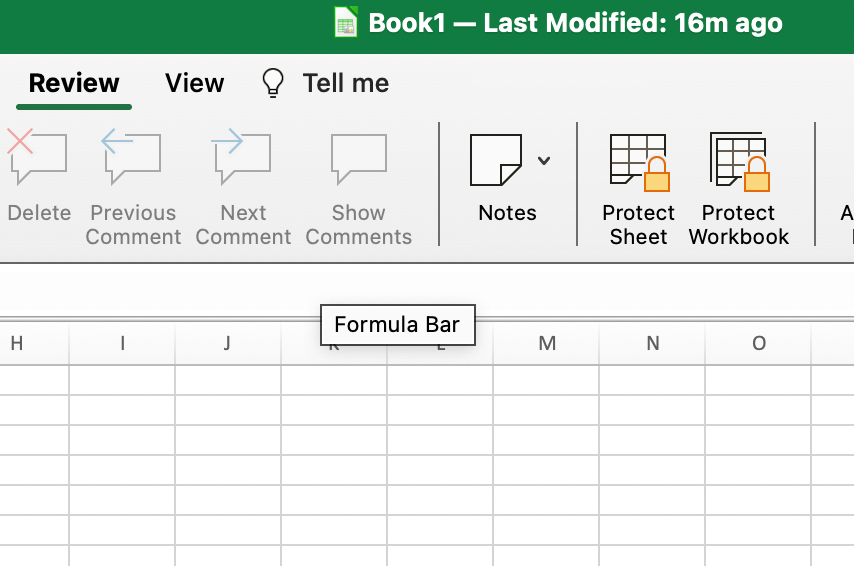
\includegraphics[width=10cm]{protectWorkbook.png}
			\end{center}
	\end{frame}
	\section{AutoFit and AutoFill}
	\begin{frame}
		\frametitle{AutoFill}
		AutoFill recursively applies cell functions while dragging cursor down a row or column. e.g., 
		\begin{itemize}
			\item 1,2,3,4, \ldots
			\item 5,10,15, \ldots
			\item January, February, March, \ldots
			\item Sunday, Monday, Tuesday, \ldots
		\end{itemize}
	\end{frame}

	\begin{frame}
		\frametitle{AutoFit}
		Automatically enlarges or shrinks a column to fit its content to fit the widest entry:
		The action is performed by
		\begin{itemize}
			\item double-clicking the right edge of a column header to resize the column.
			\item double-clicking the bottom edge of a row header to resize the row.
		\end{itemize} 
		
	\end{frame}
	\begin{frame}
		\frametitle{Undo and Redo \& External Reading}
		Excel tracks the last 100 actions.
		Undo/Redo buttons are found on the far left hand side of the ribbon in Office 365. \\
		\bigskip
		Keyboard short cuts for undo and redo are Ctrl (Cmd) + Z, and Ctrl (Cmd) + Y, respectively.
		
		\bigskip
		Check out the appendix of ``Introduction to Statistics through resampling and Microsoft Office Excel".
		
	\end{frame}
	
\end{document}





